\documentclass[a4paper,article,oneside]{memoir}
    \title{\textbf{Bug Reporting}}
    \author{Justal Kevin}
    \date{1 May 2022}
    
    \addtolength{\topmargin}{-3cm}
    \addtolength{\textheight}{3cm}
\usepackage[latin1]{inputenc}
\usepackage[T1]{fontenc}
\usepackage{graphicx}
\graphicspath{ {./images/} }
\usepackage[acronym]{glossaries}
\usepackage{tabularx}
\usepackage{verbatimbox}
\usepackage[dvipsnames]{xcolor}
\makeglossaries

\newglossaryentry{PO}
{
        name=PO,
        description={Is a Product Owner}
}

\newglossaryentry{PM}
{
        name=PM,
        description={is a Product Manager}
}

\newglossaryentry{Business}
{
        name=Business,
        description={is any person from the sales teams}
}

\newglossaryentry{QA}
{
        name=QA,
        description={is any person from the quality assurance teams}
}

\newglossaryentry{DEV}
{
        name=DEV,
        description={is any person responsible for the development of the features}
}

\newglossaryentry{TL}
{
        name=TL,
        description={is the team leader of the backend or frontend team}
}

\newglossaryentry{FT}
{
        name=FT,
        description={is the frontend team}
}

\newglossaryentry{DT}
{
        name=DT,
        description={is the data team}
}

\begin{document}
\maketitle
\thispagestyle{empty}
\renewcommand{\contentsname}{Table of contents}
\tableofcontents*
\part{How to report a bug on Slack and Jira}
	\chapter*{Preface}
	\addcontentsline{toc}{chapter}{Preface}
		When reporting a bug, there are some mandatories information in order for anyone to understand and fix rapidly any problem. The following points are the minimum required for any bug ticket :
	
        \begin{enumerate}
  			\item {\color{BrickRed}\textbf{Title}}
  			\item {\color{BrickRed}\textbf{Description}}
  			\item {\color{BrickRed}\textbf{Replication}}
  			\item {\color{BrickRed}\textbf{Screenshots}}
		\end{enumerate}
		
	You will find below more explanation about each point with some examples directly taken from Jira.
		\chapter{Title}
		The title is the first thing we see when looking at a ticket. It should be short, precise and concise. Anyone from the team should be able to understand the problem just by reading it. If the titles are correctly set, we can also use the filters of Jira for finding the tickets related to each other.
		
\noindent\addvbuffer[12pt 8pt]{{\color{ForestGreen}\underline{For example :}}}

\begin{itemize}
  \item Data Integration: User redirect to login page when clicking connection to google drive
  \item STAGE: Action Micro: get\_action\_by\_id returning an error inside commitment step
\end{itemize}

\noindent\addvbuffer[12pt 8pt]{{\color{BrickRed}\underline{Bad example:}}}

\begin{itemize}
  \item CONNEC
  \item Unable to recall variables
  \item Create the new Factors
\end{itemize}
	
		
        \chapter{Description}
        In the description, the bug should be describe as simple as possible for anyone to be able to understand it. It needs to be exhaustive, the more information the better, the more information the easier it is to understand the problem. The bug should not be only understandable by the one handling the ticket/bug. The reason is simple, what happen if the reporter and the one handling the ticket are not in position for answering (Holiday, hospital...). In this case, the ticket need to be handle by someone else and he will need to understand the problem without any external help.
        
\noindent\addvbuffer[12pt 8pt]{{\color{ForestGreen}\underline{For example :}}}

When passing edit user types payload for permissions it needs to pass as an array but
when passing the create user types payload it needs to be passed as a string instead of an array

conclusion the schema for both edit user types permission and create user types payload permissions should be the same

\noindent\addvbuffer[12pt 8pt]{{\color{BrickRed}\underline{Bad example:}}}  

\begin{itemize}
  \item Defect on Add Company
  \item see screenshot for more info
  \item Or even worse a ticket without description
\end{itemize}
     
        \section{Replication}
        This section is certainly the most important. Every step for replicating the bug should be describe. It's really hard and in some cases impossible for the developers to find why the system is returning an error. So helping the developers by providing a step by step will make the problem easy to find and of course, will decrease by a lot the time needed for fixing bugs. It's a win-win for everyone.

\noindent\addvbuffer[12pt 8pt]{{\color{ForestGreen}\underline{Good example :}}}

\begin{itemize}
  \item Click FB icon on login page
  \item Enter incorrect username
  \item Click Add username
  \item Enter enter company
  \item Click Add Company
  \item Enter "sd da"
  \item Click Create Account
  \item {Should display

"A username cannot contain white space or be more than 32 characters"

Actual:

"An username cannot contain white space or be more than 32 characters"}
\end{itemize}

\noindent\addvbuffer[12pt 8pt]{{\color{BrickRed}\underline{Bad example:}}}

The current recommender system doesn't work. it recommends the same set of actions no matter what the keywords is.

        \section{Screenshots}
        A description should always been accompagned with a screenshoot. Text alone is often not enough for pin-pointing where is the problem. Human are visual creature, so a text plus an image made any bug reported clearer. It also limits the scope of the error to what the screenshot will show.
        
        This section is mandatory for any visual bug. The buggy part or the problem should be hightlighed on the screenshot by making a red circle around the area where the problem is.

If any screenshot of queries or mutations are made, those queries/mutations should also be written in the ticket in the description part. You already took the time to write the queries, so make it easier for the next developers. Copy/paste your queries for him to just use it and not rewritting everything from a picture.
        
\noindent\addvbuffer[12pt 8pt]{{\color{ForestGreen}\underline{For example :}}}

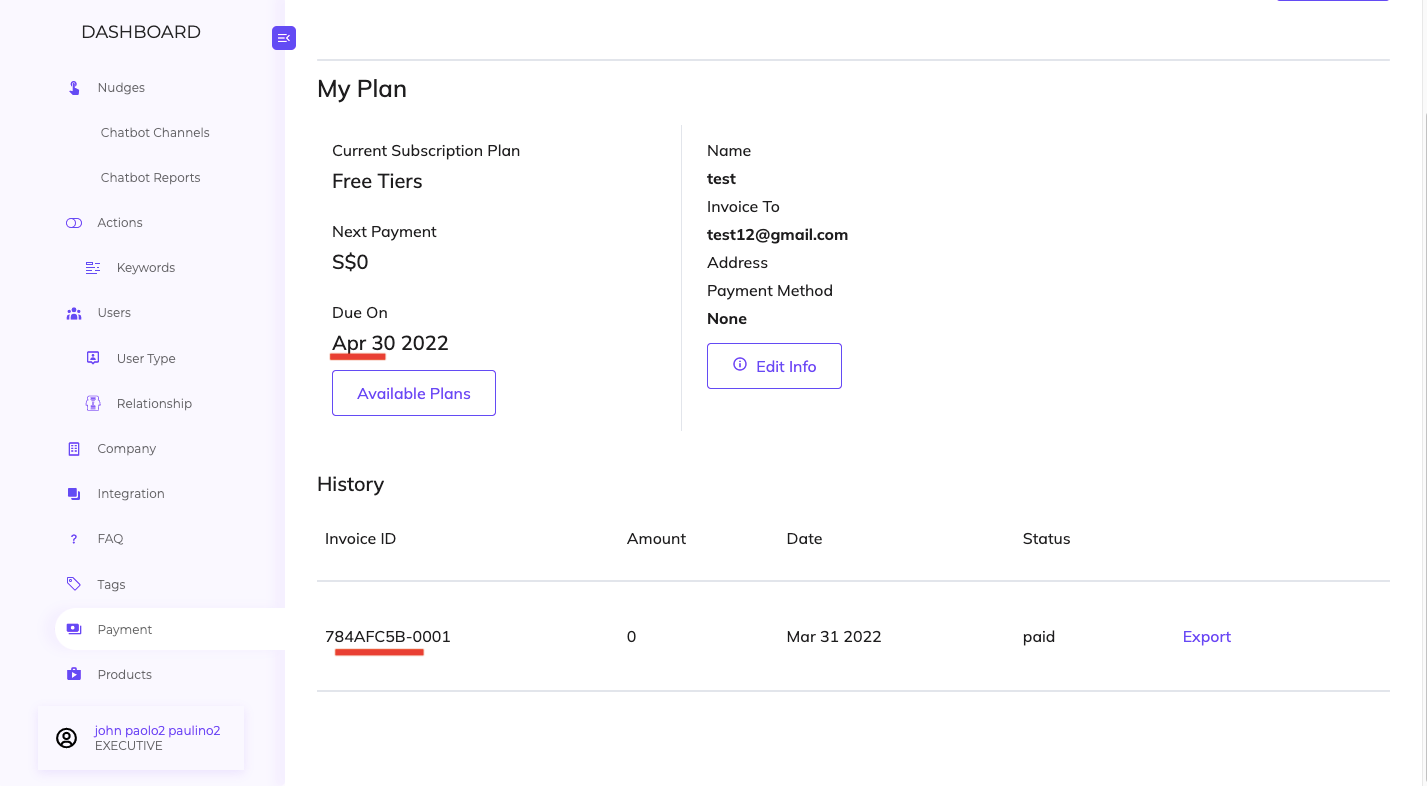
\includegraphics[width=\textwidth]{3}

\noindent\addvbuffer[12pt 8pt]{{\color{BrickRed}\underline{Bad example:}}}  

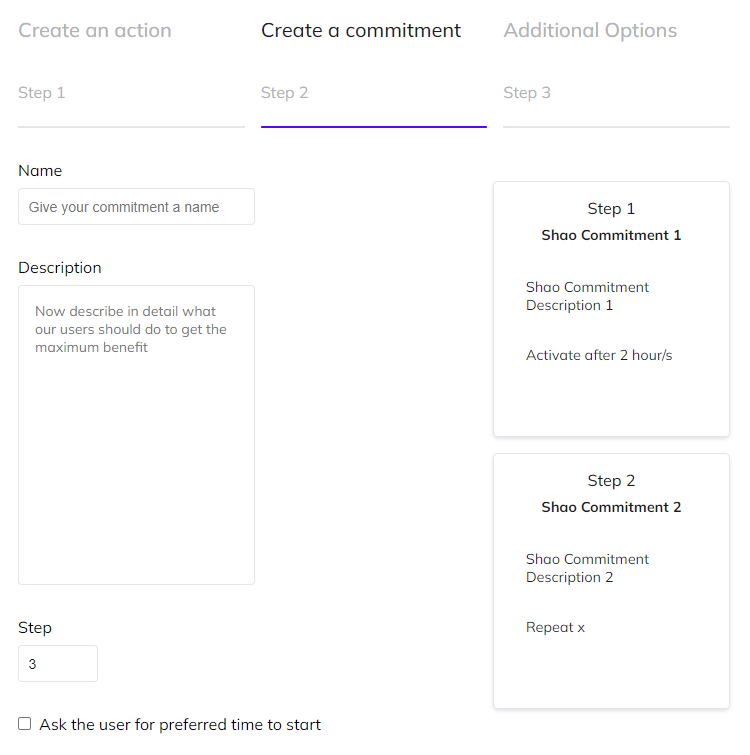
\includegraphics[width=\textwidth]{2}

\printglossary[nonumberlist]
\end{document}